\startchapter{Theory}
\label{chapter:theory}

\newlength{\savedunitlength}
\setlength{\unitlength}{2em}

The \textbf{Standard Model of Particle Physics (SM)} is a quantized relativistic field theory that describes all known elementary particles, as well as their interactions via three of the four known fundamental forces. It has been tested extremely rigorously since its development in the 1960s and 1970s, and in every case its predictions have held true. The final piece of the puzzle fell into place in 2012 with the experimental verification of the existence of the Higgs Boson in 2012. (cite https://www.sciencedirect.com/science/article/pii/S037026931200857X).

Despite its success, however, the SM is considered an incomplete theory. It does not describe the interaction of matter via the fourth fundamental force, gravity, nor does it account for the existence of \textit{dark matter} in our universe, or the asymmetry between the observed amounts matter and anti-matter. These shortcomings provide motivation to extend the SM by searching beyond it for new phenomena.

This chapter will provide a short overview of the SM theory, before describing some of the deficiencies that motivate extending it.

\section{The Standard Model}

\subsection{The Particles}
The elementary particles of the Standard Model are shown in Figure \ref{fig:standardmodel}. They can be categorized into two groups: \textit{fermions} and \textit{bosons}. \textit{Fermions} carry half-integer spin, and constitute the matter that surrounds us. For each fermion there also exists a corresponding anti-particle with an opposite electric charge. In this document anti-particles will be denoted either by the charge (e.g. $e$ vs. $e^{-}$) or by a bar overhead e.g. ($t$ vs. $\bar{t}$). The fermions can be further divided into two groups: \textit{leptons} and \textit{quarks}. \textit{Leptons}, the most familiar of which is the electron, interact via the weak force and, if electrically charged, the electromagnetic force. They come in three flavour generations, each of which has a neutral particle (\textit{neutrino}) and a charged fermion with charge -1. Unlike leptons, which regularly exist freely, \textit{quarks} exist mostly in bound states called \textit{hardrons}, the most well-know of which are the proton and neutron composed of ($u,u,d$) and ($u,d,d$) quarks respectively. Like leptons, quarks come in three generations, each of which has a pair of particles with electric charges +2/3 and -1/3. They interact via all three forces of the standard model: strong, weak, and electromagnetic.

\begin{figure}[h]
    \centering
    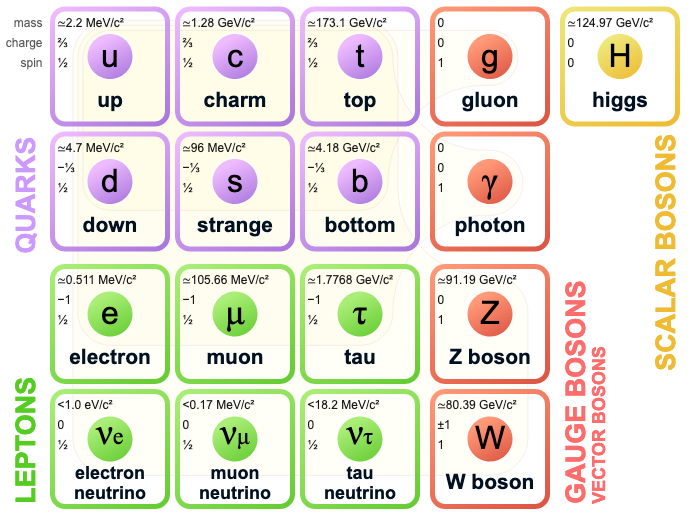
\includegraphics[width=0.8\textwidth]{Figures/1/sm.png}
    \caption{The elementary particles of the Standard Model}
    \label{fig:standardmodel}
\end{figure}

\textit{Bosons} carry integer spin, and mediate the forces via which particles interact. Massless \textit{gluons} and \textit{photons} as well as massive W and Z bosons are spin-1 vector bosons, while the Higgs Boson is a spin-0 scalar boson. The massive W and Z vector bosons are the carriers of the weak force, the photon carries the electromagnetic force, and the gluons carry the strong force binding quarks. Along with interacting with fermions via exchange, bosons are also able to interact among themselves. $W$ bosons are able to directly interact with both $Z$ bosons and and photons, as well as self-interacting. Gluons can also self-interact, but $Z$ bosons and photons cannot. The Higgs boson interacts with all massive particles, including self-interaction, and it is via their interaction with the Higgs field that massive bosons obtain their mass.

\subsection{Quantum Electrodynamics (QED)}
\textit{Quantum Electrodynamics} (QED) is a quantum field theory of electrodynamics and the electromagnetic force. It describes the interaction of electrically charged particles via the exchange of photons. Mathematically, QED is an abelian (commutative) gauge theory with the gauge group $U(1)$. The fundamental interactions of the theory are: the emission or absorption of a single photon by a charged particle and the creation or annihilation of a pair of charged particles. These interactions can all be represented by various orientations of the Feynman vertex shown in Figure ~. 

\subsection{Weak Interactions}
The weak force, in contrast to the electromagnetic force, is mediated by the exchange of massive vector bosons $W^+$, $W^-$, and $Z$. Owing to the charge of the W bosons, and the fact in contrast to the electromagnetic force neutral fermions also interact via the weak force, there are many more possible fundamental interactions. Figure ~ shows the vertices corresponding three such interactions: Fermions interacting with the $Z$ boson in a similar vertex to that of Figure ~ shown in (a), a charged lepton and neutrino interacting with a $W$ boson shown in (b), and a quark-antiquark pair interacting with a $W$ boson shown in (c).

At high energy scales, the aforementioned electromagnetic force and the weak force unify to become the electroweak interaction. Glashow, Salam, and Weinberg's theory unites to two forces into a single $U(1) \bigotimes SU(2)$ gauge theory. 

\subsection{Quantum Chromodynamics (QCD)}
\textit{Quantum Chromodynamics} (QCD) is the theory describing the strong interaction between gluons and quarks. It is again a gauge theory, this time with the SU(3) symmetry group. There are three colour charges associated with this group, which are carried by both quarks and gluons. Each of the 8 gluons carries a unique colour charge and anti colour charge pair, while quarks carry a single colour charge. Because they carry colour charge, gluons are able to both interact with quarks and self-interact. This gives rise to several possible interaction vertices in the theory, some of which are shown in Figure ~.

\subsection{The Higgs Boson}
Electroweak theory and QCD alone do not allow any massive particles. In these theories, it is possible to go beyond single-particle exchanges to multi-particle exchanges. The amplitude of these exchanges is computed as an integral over the momenta of the exchanged particles. These integrals often diverge as the momenta of the exchange particles approaches infinity. The theory is saved, however, by \textit{renormalization}, which counters the divergences. If particles were to have a mass term in the Lagrangian of the theory, however, the energy scale of the theory would be fixed, and renormalization would no longer be possible.

\section{Beyond the Standard Model}









































Here is where you tell me what is the problem you have been working on for the past few months (or years). I want all the details and you should not be timid about being too tutorial, except that you do not want to cross the line towards writing a textbook. However consider carefully that \textit{communication} implies conveying ideas to other people, while \textit{effective communication} occurs when your message is clearly understood. Remember that your audience must understand your message before they can agree with you.

Ask yourself:
\textit{who is your audience?} You might think of your supervisor who knows everything and you want to impress with your knowledge. I think instead of the graduate students who will be reading this thesis which is, after all, a property of the university. It is published as a university technical report so that others may learn by reading it. Then teach them! Be a bit tutorial. Even the expert external examiner will be impressed by your clarity of exposition if he or she does not need to read paragraphs twice in order to understand - something which people with PhDs and big egos find particularly irritating.

On the other hand, do not go too far and give trivial definitions from concepts learned in a 3rd year undergraduate courses, else you might find yourself in trouble when having to remember the details during an oral examination.

My approach is to put everything necessary to make clarity for
the problem the main goal of this chapter, assuming an intelligent and well prepared reader who already has a Bachelor degree in an appropriate subject.

Once I understand the problem clearly and its nuances (it may not be what I expected after all), I also need to know why the problem is important, what its impact is and what its application, if any. Here you are free to elaborate and write as much as you think is necessary to avoid the examination doubt that you have a brilliant new solution to a trivial and unimportant issue.

I suggest reading various books on how to do research and set up problems. The best for me was "The Craft of Research" by Wayne Booth \cite{booth1}, which can be found in the main library at Q180.55 M4B66. From there I have transferred to my writing a fairly simple structure for talking about the topic of the research, with the question to be asked and its motivation and significance. It goes as follows:
\begin{enumerate}
\item {\textit{I am trying to learn about (working on, studying...)}}
\item {\textit{because I want to find out....}}
\item {\textit{in order to understand...}}
\end{enumerate}

Another way of looking at this is to ask the
\textit{what}, \textit{why} and \textit{where}, starting from a \textit{setting} of the problem with a first point A, stating what the \textit{goal} is at point B and having an \textit{action link} between the two which will encompass your new solution. As surprising as this may be to some of you, I found reading a book from Microsoft very useful: "Beyond Bullet Points: Using Microsoft Office PowerPoint 2007 to Create Presentations That Inform" \cite {atkin}. The goal of the book is to improve presentations with Power Point, but there is a lot that can be transferred towards \textit{effective communication} for a thesis.

In summary, my view of the second chapter on
\textit{"The Problem to be solved"} is as follows:
\begin{enumerate}
\item {\textit{Not} all the background and definitions (boring!) - use instead just-in-time explanations as needed in every context as it comes up;}
\item {Motivation in depth;}
\item {Tutorial high level explanation, where it is important to choose the right pitch: who is the audience? who are you teaching here?}
\item {Make it exciting, make it current, make it important - why do I want to keep reading?}
\item {Should you list here the solutions from other researchers? I think not, list instead the different facets of the problems that other researchers have attacked.}
\item {A taxonomy can be extremely useful to place your problem and its particular special features within the perfect context of the overall area, as you need to make sure that the reader understands perfectly what you are trying to solve.}
\end{enumerate}


\setlength{\unitlength}{\savedunitlength}
